\documentclass[a4paper,11pt]{report}
\usepackage[T1]{fontenc}
\usepackage[utf8]{inputenc}
\usepackage{lmodern}
\usepackage[francais]{babel}
\usepackage[usenames,dvipsnames,svgnames,table]{xcolor}
\usepackage[colorlinks,linkcolor={blue!30!black},citecolor={blue!50!black},urlcolor={blue!80!black}]{hyperref}
\usepackage{amsmath,array,graphicx,caption,lmodern,subcaption,tikz,url,xspace,wrapfig}
\usepackage{textcomp,rotating,pdfpages}
\usepackage{epic,eepic}
\usepackage[top=2cm,left=2.5cm,right=2.5cm,bottom=2cm]{geometry} % Géométrie de la page, modifier selon le besoin
\usepackage[babel=true,kerning=true]{microtype}
\usepackage{float}
\usepackage{textcomp}
\usepackage{newfloat}
\usepackage{fancyhdr}
\lhead{}
\chead{}


\DeclareFloatingEnvironment[fileext=frm,placement={!ht},name=Tableau]{tableau}
\captionsetup[tableau]{labelfont=bf}

% \pdfsuppresswarningpagegroup=1
\title{Rapport de Stage d'Application}


\begin{document}
\pagenumbering{gobble}  % Pas de numérotation
\begin{titlepage}
    \vspace*{50px}
    
\includegraphics[height=80px]{Images/logo_phelma.pdf}
    \vspace*{-80px}
\begin{flushright}
%     \vspace*{60px}
    
\includegraphics[height=65px]{Images/CIME.jpg}
\end{flushright}

\vspace*{2cm}

\begin{center}
\rule{\linewidth}{0.5mm}\\[0.4cm]
{\huge{\bfseries Compte Rendu}\\[0.4cm]
\textsc{TP Simulation électronique}\\[0.4cm]}
\rule{\linewidth}{0.5mm}\\[0.5cm]

\LARGE{\textsc{Nicolas Paillet, Félix Piédallu \& Giulia Rizzo}}\\[0.7cm]
\large{\textsc{2015-2016}}\\[2cm]

\Large{~}\\[1cm]
% 
\includegraphics[width=0.4\textwidth]{Images/CIME.jpg}\\[1cm]
%
 \large{Encadrant : Marco Pala}\\[2cm]
%

\end{center}
\end{titlepage}

\tableofcontents        % Table des matières avec liens, générée automatiquement.
\newpage
\pagenumbering{arabic}  % Numérotation de retour !


\chapter*{Introduction}
\addcontentsline{toc}{chapter}{Introduction}
Lors de la conception de composant à semiconducteurs, il est important d'avoir des outils de simulation pour avoir une idée des résultats et performances attendues. Il est également important de maîtriser ces outils de simulation pour réaliser ces simulations. Ce TP a pour but de nous initier à certains de ces outils en nous proposant de réaliser la simulation de composants MOS tel que ceux étudiés de manière théorique en cours, via la suite logicielle Silvaco. Ainsi, nous pourrons observer des graphes numériques sur les équations calculées théoriquement, mais également comparer différentes architectures de composants et même observer des représentations du champs à l'intérieur des transistors en fonctionnement.

\chapter{Architecture "Bulk"}

\section{Position du problème}
Dans cette partie, on cherche à modéliser un transistor dit "Bulk", que l'on peut représenter schématiquement (Figure \ref{SchemaBulk})
\begin{figure}[H]
    \centering
    \begin{tikzpicture}
        \fill [color=gray!20] (3,5)--(7,5)--(7,4.8)--(3,4.8)--cycle;
        \fill [color=black] (3,5)--(7,5)--(7,5.2)--(3,5.2)--cycle;
        \draw [thick] (0,5)--(10,5);
        \draw (3,5)--(3,3)--(0,3);
        \draw (1.5,4)node{n};
        \draw (7,5)--(7,3)--(10,3);
        \draw (8.5,4)node{n};
        \draw (5,4.8)node[below]{Canal};
        \draw (3,5)--(3,6)--(7,6)--(7,5)--cycle;
    \end{tikzpicture}
    \caption{Schéma d'un transistor Bulk}
    \label{SchemaBulk}
\end{figure}
\section{Initialisation de la simulation}

Tout d'abord, on utilise l'éditeur \texttt{deckbuild} afin de mettre en place la séquence de commandes à réaliser dans le logiciel \texttt{Atlas}. En premier lieu il faut créer un maillage 2D pour pouvoir y inclure des régions.
\vspace{0.3cm}

\noindent\fbox{
\begin{minipage}{\textwidth}
    \noindent\texttt{go atlas\\
    mesh space.mult = 1.0\\
    x.mesh loc=0.0 spac=0.001\\
    x.mesh loc=0.1 spac=0.001\\
    x.mesh loc=0.2 spac=0.001\\
    x.mesh loc=0.3 spac=0.001\\
    y.mesh loc=0.000 spac=0.0001\\
    y.mesh loc=0.002 spac=0.0001\\
    y.mesh loc=1.002 spac=0.01}
\end{minipage}}
\vspace{0.3cm}

Il faut ensuite dessiner le composant que nous voulons modéliser sur cette grille. Pour cela, il nous suffira de dessiner des régions en précisant les matériaux utilisés pour chacune d'entre elles.
\vspace{0.3cm}

\noindent\fbox{
\begin{minipage}{\textwidth}
\noindent\texttt{region number = 1 x.min=0.0 x.max = 0.3 y.min = 0.0 y.max = 0.002 material = Oxide\\
region number = 2 x.min=0 x.max = 0.3 y.min = 0.002 y.max = 1.002 material = Silicon}
\vspace{0.3cm}

\noindent\texttt{electrode name = gate   number = 1 x.min = 0.1 x.max = 0.2 y.min = 0.00 y.max = 0\\
electrode name = source number = 2 x.min = 0.0 x.max = 0.0 y.min = 0.002 y.max = 0.012\\
electrode name = drain  number = 3 x.min = 0.3 x.max = 0.3 y.min = 0.002 y.max = 0.012}
\vspace{0.3cm}

\noindent\texttt{doping uniform conc = 1E15 p.type region = 2\\
doping uniform conc = 1E20 N.type region = 2 x.left = 0.0 x.right = 0.1 y.max = 0.012\\
doping uniform conc = 1E20 N.type region = 2 x.left = 0.2 x.right = 0.3 y.max = 0.012\\
struct outf = mos.str}
\end{minipage}}
\vspace{0.3cm}

\begin{figure}[H]
\centering
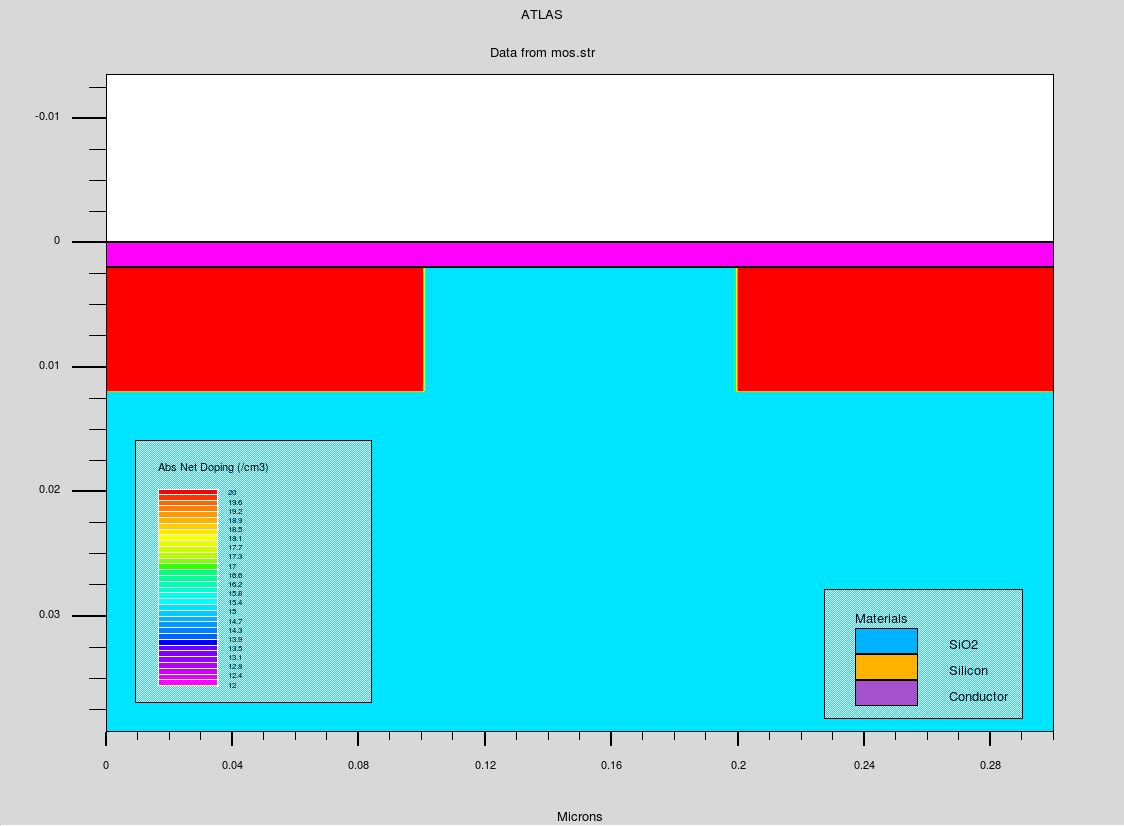
\includegraphics[width=300pt]{Images/Simu1-Dopage.png}
\caption{Image des différentes régions et dopages générés par le logiciel}
\label{transistortonyplot}
\end{figure}

Nous avons ainsi une modélisation 2D du transistor, comme le montre la Figure \ref{transistortonyplot}.

On précise ensuite au logiciel les différents contacts que nous allons utiliser, on obtient ainsi l'image en Figure \ref{TransistorFull}

\begin{figure}[H]
    \centering
    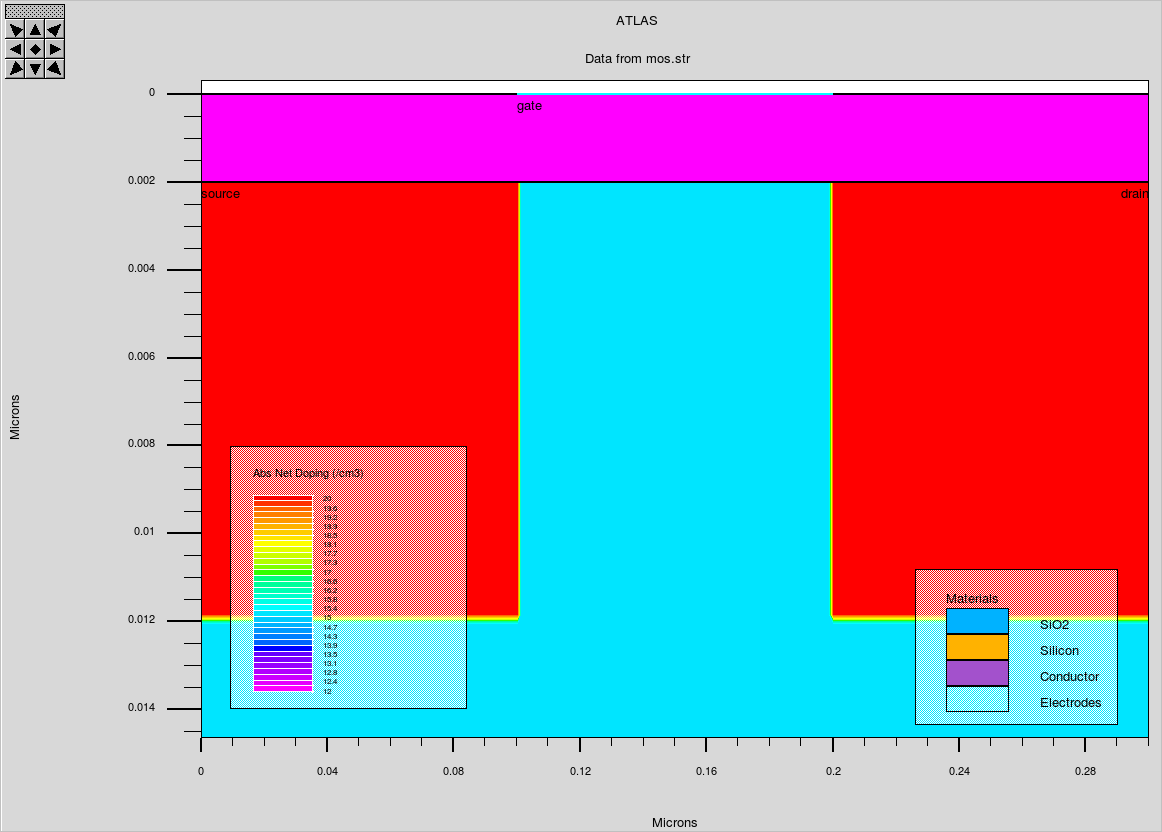
\includegraphics[width=300pt]{Images/TransistorFull.png}
    \caption{Image des régions, du dopage ainsi que des contacts générée par le logiciel}
    \label{TransistorFull}
\end{figure}

Maintenant que notre transistor est modélisé, nous allons pouvoir réaliser des simulations en jouant avec les différentes tensions appliquées.

\section{Tracés de caractéristiques}

En effet, il suffit ensuite d'ajouter quelques lignes au script afin de tracer des courbes, comme le montre la figure \ref{logIdVgmeshfin}.

\noindent\fbox{
\begin{minipage}{\textwidth}
    \noindent\texttt{output charge band.param ex.field ey.field jx.tot con.band val.band}
    \vspace{0.3cm}

    \noindent\texttt{solve init\\
    save outfile = nmos1.str}
    \vspace{0.3cm}

    \noindent\texttt{solve vgate = 0 vdrain = 0 vstep = 0.1 vfinal = 1 name = drain\\
    save outfile = nmos2.str}
    \vspace{0.3cm}

    \noindent\texttt{log outfile = idvg\_vds1.log\\
    save outfile = nmos3.str\\
    solve vgate = 0 vdrain = 1 vstep = 0.1 vfinal = 2 name = gate\\
    extract name="vt" (xintercept(maxslope(curve(abs(v."gate"),abs(i."drain")))) \ }

    \hspace{1cm} \texttt{- abs(ave(v."drain"))/2.0)}\\
    \texttt{extract name="subvt" \ }

    \hspace{1cm} \texttt{ 1.0/slope(maxslope(curve(abs(v."gate"),log10(abs(i."drain")))))}
\end{minipage}}

\begin{figure}[H]
\centering
    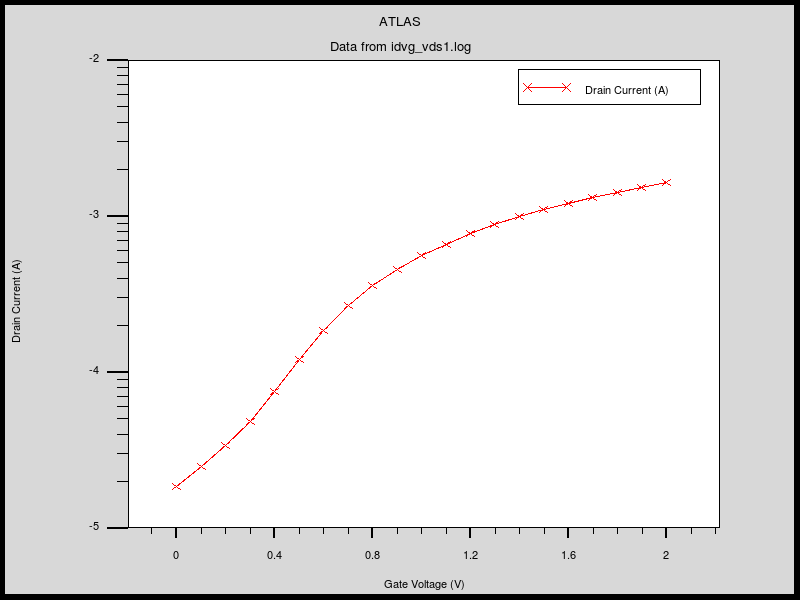
\includegraphics[width=300pt]{Images/MeshFin.png}
    \caption{Caractéristique logarithmique $\log(I_d(V_g))$}
    \label{logIdVgmeshfin}
\end{figure}


% Il est également possible de tracer la caractéristique $I_d(V_d)$
%Graphe

A partir de ce graphe il est possible d'extraire différents paramètres. Par exemple, pour $V_{ds}=50mV$, on trouve, pour la tension de seuil, la pente sous le seuil, le courant de saturation et le courant à vide :

\begin{tableau}[H]
\centering
\begin{tabular}{|c|c|}
\hline
$V_t$&$500mV$\\
\hline
$SubV_t$&$170mV/decade$\\
\hline
$I_{sat}$&$20mA$\\
\hline
$I_{off}$&$20\mu A$\\
\hline
\end{tabular}
\caption{Caractéristiques avec un maillage fin pour $V_{ds}=50mV$}

\end{tableau}



\section{Optimisation du maillage}

Nous avons pu voir lors des calculs précédents qu'avec le maillage proposé initialement, l'obtention de points est très longue. En effet, le maillage est beaucoup trop fin, en particulier à des endroits où il n'a pas besoin de l'être. Par exemple le maillage n'a pas besoin d'être précis loin en profondeur, ni loin des interfaces. Par contre, proche des interfaces il faut qu'il soit fin pour bien représenter les changements brusques.
 
\vspace{0.3cm}

On modifie alors le maillage comme suit :
\vspace{0.3cm}

\noindent\fbox{
\begin{minipage}{\textwidth}
    \noindent\texttt{mesh space.mult = 1.0\\
    x.mesh loc = 0.0 spac = 0.005\\
    x.mesh loc = 0.1 spac = 0.001\\
    x.mesh loc = 0.2 spac = 0.001\\
    x.mesh loc = 0.3 spac = 0.005\\
    y.mesh loc = 0.000 spac = 0.0001\\
    y.mesh loc = 0.002 spac = 0.001\\
    y.mesh loc = 0.020 spac = 0.01\\
    y.mesh loc = 1.002 spac = 0.01}
\end{minipage}}
\vspace{0.3cm}

On peut ainsi également tracer la caractéristique obtenue avec ce maillage, en figure \ref{logIdVgmeshopti}

\begin{figure}[H]
    \centering
    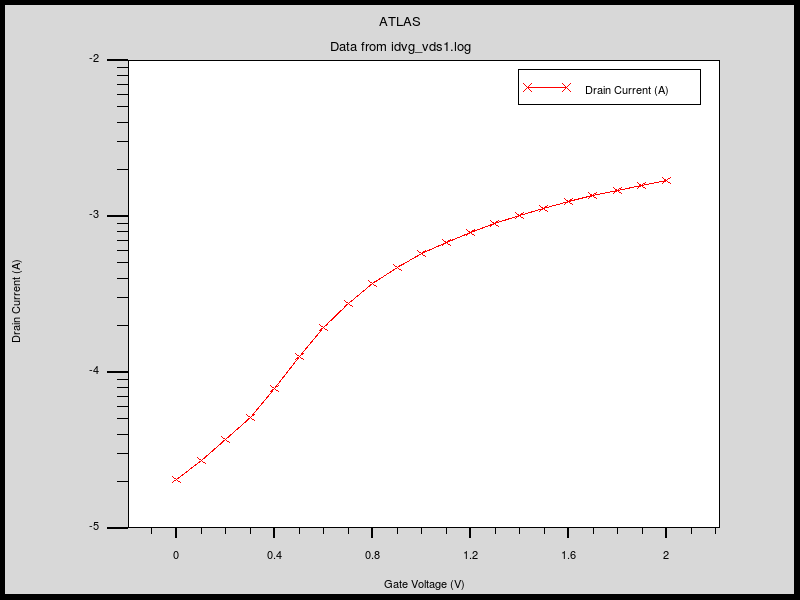
\includegraphics[width=300pt]{../meshOpti1/Log.png}
    \caption{Caractéristique $\log(I_g(V_g))$ obtenue avec un maillage optimisé.}
    \label{logIdVgmeshopti}
\end{figure}

On peut également extraire des paramètres de ce tracé, comme avec le maillage fin. On trouve ainsi :

\begin{tableau}[H]
\centering
\begin{tabular}{|c|c|}
\hline
$V_t$&$500mV$\\
\hline
$SubV_t$&$170mV/decade$\\
\hline
$I_{sat}$&$20mA$\\
\hline
$I_{off}$&$22\mu A$\\
\hline
\end{tabular}
\caption{Caractéristiques avec un maillage optimisé avec $V_{ds}=50mV$}
\end{tableau}

Les valeurs trouvées sont cohérentes avec les valeurs précédentes, ce qui laisse à penser que le maillage optimisé ne réduit pas la précision

Il convient ensuite de comparer les deux courbes obtenues, pour vérifier si le maillage moins précis donne le même résultat que le maillage fin. Cette comparaison est fournie en Figure \ref{compMesh}

\begin{figure}[H]
  \centering
  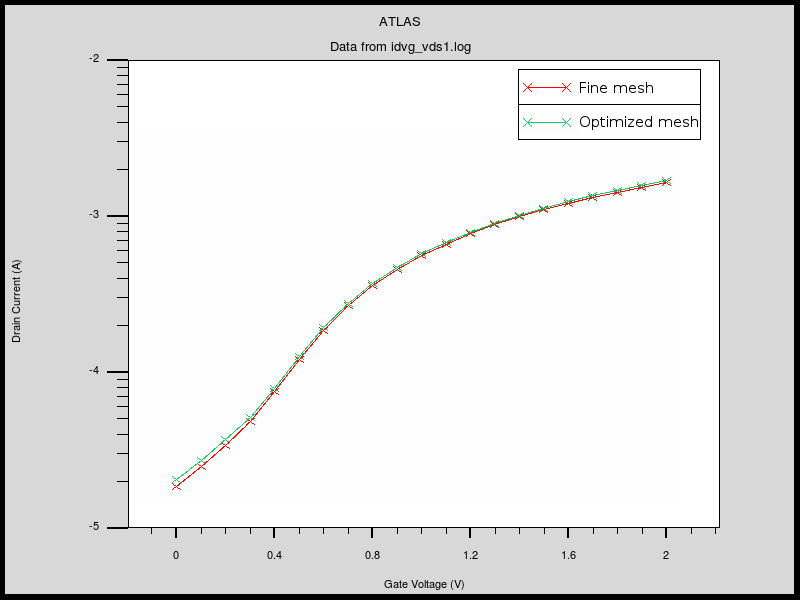
\includegraphics[width=250pt]{Images/MeshFinEtOpti.png}
  \caption{Comparaison des deux maillages pour $V_{ds}=50mV$}
  \label{compMesh}
\end{figure}

\section{Extraction des paramètres}
A partir des caractéristiques tracées, nous pouvons remonter à certains paramètres. Par exemple, SS et DIBL.

%SS 

%DIBL


\chapter{Une autre architecture : FDSOI}

\section{Position du problème}

On passe à une architecture Fully Depleted Silicon On Insulator (FDSOI), qui permet de limiter la variation de $V_t$ avec la réduction de la longueur de grille, qui apparaît avec l'architecture Bulk.  Le schéma représentant cette architecture est donné en Figure \ref{SchemaFDSOI}.

\begin{figure}[H]
    \centering
    \begin{tikzpicture}
        \fill [color=gray!20] (3,5)--(7,5)--(7,4.8)--(3,4.8)--cycle;
        \fill [color=black] (3,5)--(7,5)--(7,5.2)--(3,5.2)--cycle;
        \draw [thick] (0,5)--(10,5);
        \draw (3,5)--(3,3)--(0,3);
        \draw (1.5,4)node{n};
        \draw (7,5)--(7,3)--(10,3);
        \draw (8.5,4)node{n};
        \draw (5,4.8)node[below]{Canal};
        \draw (3,5)--(3,6)--(7,6)--(7,5)--cycle;
        \fill [color=gray!30] (0,1)--(0,2)--(10,2)--(10,1)--cycle;
    \end{tikzpicture}
    \caption{Schéma d'un transistor FDSOI}
    \label{SchemaFDSOI}
\end{figure}

\section{Simulation}
On reprend les élements précedents en rajoutant une zone d'oxyde sous le silicium dopé n.

On obtient ainsi le dispositif suivant :

%image de dispo


\section{Tracé des caractéristiques}

On peut ainsi tracer les caractéristiques :
\begin{figure}[H]
    \centering
    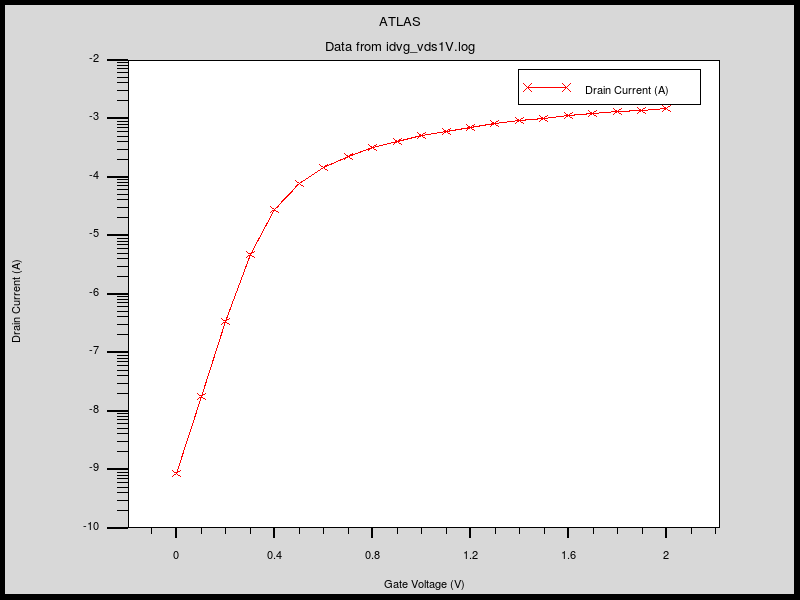
\includegraphics[width=300pt]{../FDSOI/LogIdVg.png}
    \caption{Caractéristiques $\log(I_d(V_g))$ pour $V_d$ faible (en rouge) et $V_d$ fort (en vert)}    
\end{figure}


\section{Extraction des paramètres}

De même qu'avec l'architecture précédente, on peut extraire les paramètres SS et DIBL.

%SS

%DIBL
\chapter{Architecture Bulk, Etude plus approfondie}

\section{Comparaison NMOS et PMOS}

Jusqu'à présent toutes nos études ont été réalisées sur des transistors NMOS, cependant, il est possible de voir la différence entre NMOS et PMOS en changeant les zones de dopage. 

\section{Longueur de grille}
Il est également possible de faire varier la longueur de grille des transistor pour vérifier les effets de canaux courts, donc l'évolution de $V_t$

\subsection{Comparaison des caractéristiques}

\subsection{Evolution de $V_T$}

\subsection{}

\chapter*{Conclusion}
\addcontentsline{toc}{chapter}{Conclusion}

La simulation est une grande part de la conception dans le sens où entrer quelques lignes  de code dans un programme est bien moins lourd que de mettre en place des protocoles expérimentaux de fabrication et de mesures pour des technologies novatrices dont les caractéristiques sont encore très peu connues. Cependant cela requiert des outils de simulation relativement puissant afin de modéliser tous les effets, mais aussi de solides bases théoriques qui indiquent les équations qui décrivent le comportement des dispositifs et composants. Nous avons pu observer cela via l'étude de composants relativement simples, mais dont l'étude complète et poussée est bien plus rapide via simulation que via les calculs vu en cours, ou même que via des outils de caractérisation de transistors déjà fabriqués.

\end{document}
